\documentclass{beamer}
%%%%%%%%%%%%%%%%%%%%%%%%%%%%%%%%%%%%%%%%%%%%%%%%%%%%%%%%%%%%%%%%%%%%%%%%%%%%%%%%%%%%%%%%%%%%%%%%%%
\setbeamertemplate{navigation symbols}{}
\usepackage{beamerthemeshadow}
\usefonttheme{serif}
%%%%%%%%%%%%%%%%%%%%%%%%%%%%%%%%%%%%%%%%%%%%%%%%%%%%%%%%%%%%%%%%%%%%%%%%%%%%%%%%%%%%%%%%%%%%%%%%%%
\usepackage{graphicx}
\graphicspath{ {res/} }
%%%%%%%%%%%%%%%%%%%%%%%%%%%%%%%%%%%%%%%%%%%%%%%%%%%%%%%%%%%%%%%%%%%%%%%%%%%%%%%%%%%%%%%%%%%%%%%%%%
\usepackage{polyglossia}
\setdefaultlanguage{armenian}
\setotherlanguages{english}
\usepackage{fontspec}
\newfontfamily\armenianfont{DejaVu Sans}
%%%%%%%%%%%%%%%%%%%%%%%%%%%%%%%%%%%%%%%%%%%%%%%%%%%%%%%%%%%%%%%%%%%%%%%%%%%%%%%%%%%%%%%%%%%%%%%%%%
\usepackage{minted}
\setminted[cpp]{fontsize=\footnotesize}
\setmonofont{Consolas}
%%%%%%%%%%%%%%%%%%%%%%%%%%%%%%%%%%%%%%%%%%%%%%%%%%%%%%%%%%%%%%%%%%%%%%%%%%%%%%%%%%%%%%%%%%%%%%%%%%
\usepackage{xltxtra}
\usepackage{hyperref}
%%%%%%%%%%%%%%%%%%%%%%%%%%%%%%%%%%%%%%%%%%%%%%%%%%%%%%%%%%%%%%%%%%%%%%%%%%%%%%%%%%%%%%%%%%%%%%%%%%
\usetheme{Luebeck}
\usecolortheme{crane}
%%%%%%%%%%%%%%%%%%%%%%%%%%%%%%%%%%%%%%%%%%%%%%%%%%%%%%%%%%%%%%%%%%%%%%%%%%%%%%%%%%%%%%%%%%%%%%%%%%
\definecolor{HTDark}{rgb}{0.04706, 0.13725, 0.26667} % primary color
\definecolor{HTLight}{rgb}{0.3686, 0.5255, 0.6235}   % secondary color
\setbeamercolor{palette primary}{bg=HTDark,fg=white}
\setbeamercolor{palette secondary}{bg=HTDark,fg=white}
\setbeamercolor{palette tertiary}{bg=HTDark,fg=white}
\setbeamercolor{palette quaternary}{bg=HTDark,fg=white}
\setbeamercolor{structure}{fg=HTDark} % itemize, enumerate, etc
\setbeamercolor{section in toc}{fg=HTDark} % TOC sections
\setbeamercolor{block title}{fg=white,bg=HTDark}
\setbeamercolor{block body}{fg=white, bg=HTLight}
\setbeamercolor{subsection in head/foot}{bg=HTLight,fg=white}
%%%%%%%%%%%%%%%%%%%%%%%%%%%%%%%%%%%%%%%%%%%%%%%%%%%%%%%%%%%%%%%%%%%%%%%%%%%%%%%%%%%%%%%%%%%%%%%%%%


\begin{document}

\title[Flyweight]{Նախագծման Ձևանմուշներ։ Flyweight}
\author[Հրաչյա Թանդիլյան\copyright]{Հրաչյա Թանդիլյան}
\date{2020}

%-------------------------------------------------------------------------------------------------
\begin{frame}
\titlepage
\end{frame}
%-------------------------------------------------------------------------------------------------

\section{Նպատակը}
%-------------------------------------------------------------------------------------------------
\begin{frame}\frametitle{Flyweight}
\begin{block}{Նպատակը}
    Մեծ քանակով փոքր օբյեկտներ արդյունավետ կերպով մշակելու համար կիրառել
    համատեղ օգտագործում (sharing):
\end{block}
\vfill
Նաև հայտնի է որպես
\begin{itemize}
    \item Այլ լայնորեն կիրառվող անուներ չկան:
\end{itemize}
\end{frame}
%-------------------------------------------------------------------------------------------------

\subsection{Մոտիվացիան}
%-------------------------------------------------------------------------------------------------
\begin{frame}\frametitle{Մոտիվացիան}
\begin{center}
    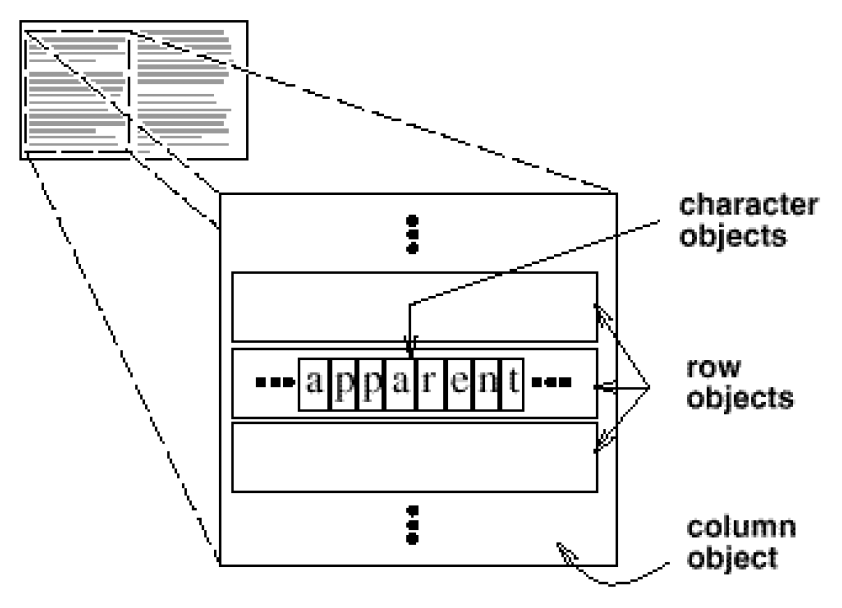
\includegraphics[scale=0.4]{motivation1.png}
\end{center}
\end{frame}
%-------------------------------------------------------------------------------------------------

%-------------------------------------------------------------------------------------------------
\begin{frame}\frametitle{Մոտիվացիան}
\begin{center}
    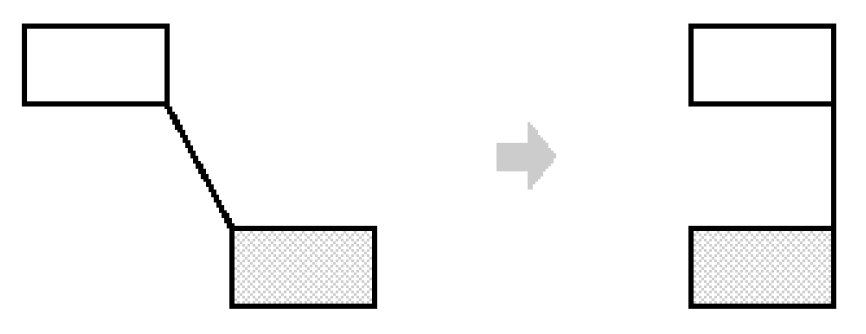
\includegraphics[scale=0.4]{motivation2.png}
\end{center}
\end{frame}
%-------------------------------------------------------------------------------------------------

%-------------------------------------------------------------------------------------------------
\begin{frame}\frametitle{Մոտիվացիան}
\begin{center}
    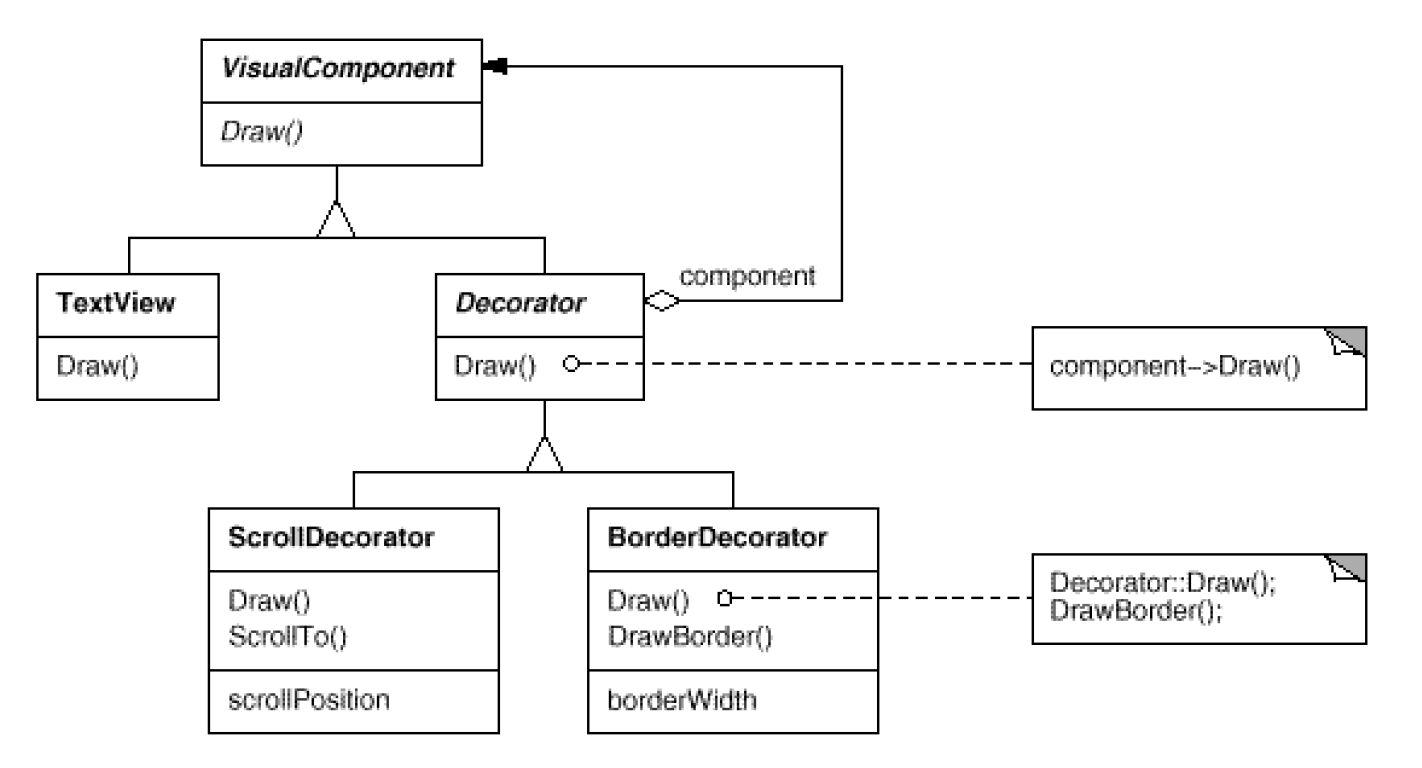
\includegraphics[scale=0.4]{motivation3.png}
\end{center}
\end{frame}
%-------------------------------------------------------------------------------------------------

%-------------------------------------------------------------------------------------------------
\begin{frame}\frametitle{Մոտիվացիան}
\begin{center}
    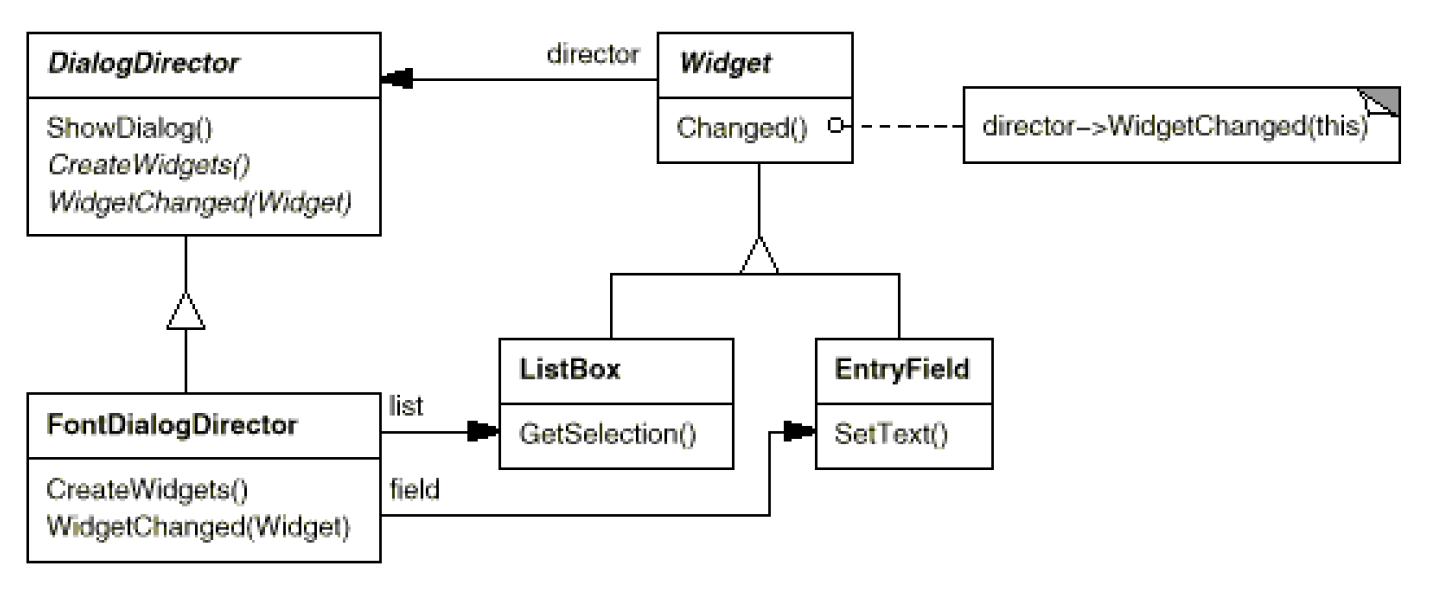
\includegraphics[scale=0.3]{motivation4.png}
\end{center}
\end{frame}
%-------------------------------------------------------------------------------------------------

\subsection{Կիրառելիությունը}
%-------------------------------------------------------------------------------------------------
\begin{frame}\frametitle{Կիրառելիությունը}
Այս Ն.Ձ. պետք է օգտագործել երբ հետևյալ բոլոր պայամանները տեղի ունեն.
\vfill
\setbeamertemplate{itemize/enumerate body begin}{\scriptsize}
\begin{enumerate}
    \item Կիրառությունը մեծ քանակով օբյեկտներ է օգտագործում: \vfill
    \item Շատ հիշողություն  է օգտագործվում, զուտ օբյեկտների քանակի մեծ
    լինելու պատճառով: \vfill
    \item Օբյեկտների վիճակների մեծ մասը կարելի է արտաքին դարձնել: \vfill
    \item Արտաքին վիճակների հեռացումից հետո օբյեկտների շատ խմբեր կարող են
    փոխարինվել համեմատաբար քիչ քանակով համատեղ օգտագործմամբ օբյեկտներով: \vfill
    \item Կիրառությունը կախված չէ օբյեկտների ինքնությունից (չի կատարում օբյեկտների
    հասցեների համեմատում):
\end{enumerate}
\end{frame}
%-------------------------------------------------------------------------------------------------

\section{Կառուցվածքը}
%-------------------------------------------------------------------------------------------------
\begin{frame}\frametitle{Կառուցվածքը}
\begin{center}
    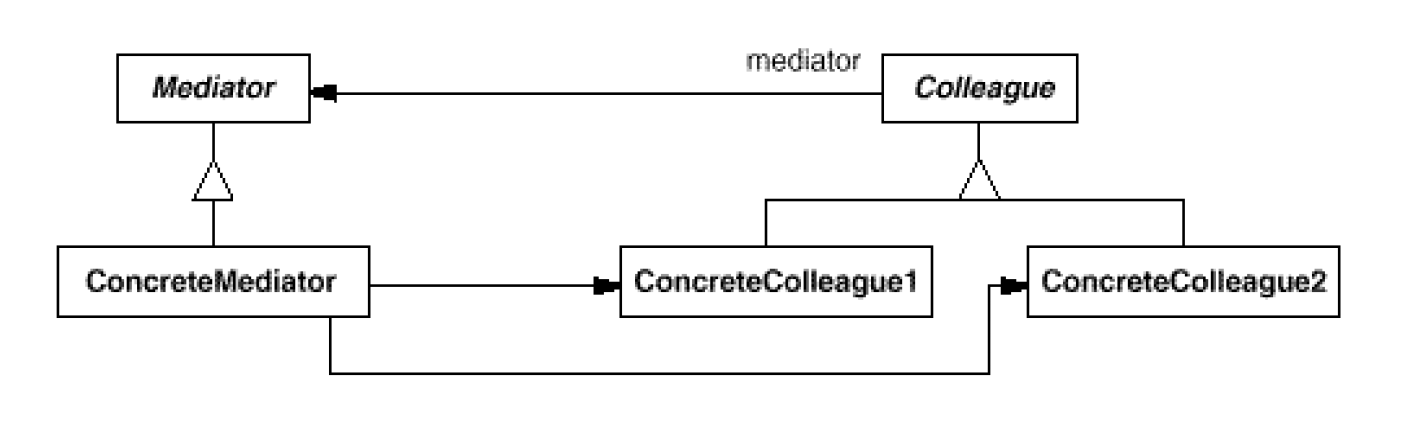
\includegraphics[scale=0.4]{structure1.png}
\end{center}
\end{frame}
%-------------------------------------------------------------------------------------------------

%-------------------------------------------------------------------------------------------------
\begin{frame}\frametitle{Կառուցվածքը}
\begin{center}
    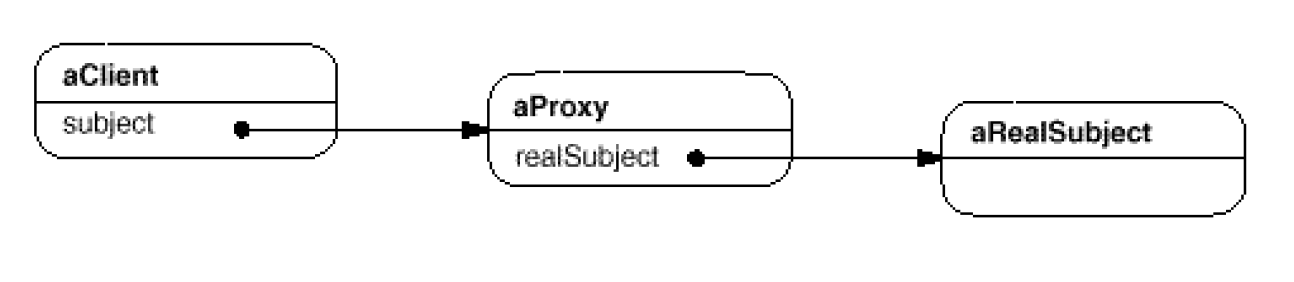
\includegraphics[scale=0.4]{structure2.png}
\end{center}
\end{frame}
%-------------------------------------------------------------------------------------------------

\subsection{Հետևանքները}
%-------------------------------------------------------------------------------------------------
\begin{frame}\frametitle{Հետևանքները}
Այս Ն.Ձ. ունի հետևյալ առավելություններն ու թերությունները.
\vfill
\setbeamertemplate{itemize/enumerate body begin}{\scriptsize}
\setbeamertemplate{itemize/enumerate subbody begin}{\scriptsize}
\begin{enumerate}
    \item Այս Ն.Ձ. կարող է առաջացնել արագության վատթարացում , որը
    լրացվում է ծախսված հիշողույան նվազեցմամբ: \vfill
    \item Հիշողության օգտագործման նվազեցումը ֆունկիցա է հետևյալ գործոններից. \vfill
    \begin{itemize}
        \item Ընդհանուր օգտագործման շնորհիվ կրճատված օբյեկտների թվաքանակից: \vfill
        \item Օբյեկտի ներքին վիճակների քանակից:
        \item Այն փաստից թե արդյոք օբյեկտի արտաքին վիճակը հաշվարկվում է, թէ պահվում: \vfill
    \end{itemize}
    \item Բերում է օգտագործված հիշողության երկակի նվազեցում: \vfill
    \item Հաճախ այս Ն.Ձ. կիրառվում է Composite Ն.Ձ. հետ համատեղ ընդհանուր
    տերևային գագաթներով գրաֆներ ներկայացնելու համար:
\end{enumerate}
\end{frame}
%-------------------------------------------------------------------------------------------------

\section{Իրականացումը}
%-------------------------------------------------------------------------------------------------
\begin{frame}\frametitle{Իրականացումը}
\begin{enumerate}
    \item Արտաքին վիճակների հեռացում: \vfill
    \item Ընդհանուր օգտագործման օբյեկտների ղեկավարում:
\end{enumerate}
\end{frame}
%-------------------------------------------------------------------------------------------------

\subsection{Օրինակ}
%-------------------------------------------------------------------------------------------------
\begin{frame}[fragile]\frametitle{Օրինակ}
\begin{english}
\begin{minted}{cpp}
class Glyph {

public:
    virtual ~Glyph();
    virtual void Draw(Window*, GlyphContext&);
    virtual void SetFont(Font*, GlyphContext&);
    virtual Font* GetFont(GlyphContext&);
    virtual void First(GlyphContext&);
    virtual void Next(GlyphContext&);
    virtual bool IsDone(GlyphContext&);
    virtual Glyph* Current(GlyphContext&);
    virtual void Insert(Glyph*, GlyphContext&);
    virtual void Remove(GlyphContext&);

protected:
    Glyph();
};
\end{minted}
\end{english}
\end{frame}
%-------------------------------------------------------------------------------------------------

%-------------------------------------------------------------------------------------------------
\begin{frame}[fragile]\frametitle{Օրինակ}
\begin{english}
\begin{minted}{cpp}
class Character : public Glyph {

public:
    Character(char);
    virtual void Draw(Window*, GlyphContext&);

private:
    char charcode;
};
\end{minted}
\end{english}
\end{frame}
%-------------------------------------------------------------------------------------------------

%-------------------------------------------------------------------------------------------------
\begin{frame}[fragile]\frametitle{Օրինակ}
\begin{english}
\begin{minted}{cpp}
class GlyphContext {

public:
    GlyphContext();
    virtual ~GlyphContext();
    virtual void Next(int step = 1);
    virtual void Insert(int quantity = 1);
    virtual Font* GetFont();
    virtual void SetFont(Font*, int span = 1);

private:
    int index;
    BTree* fonts;
};
\end{minted}
\end{english}
\end{frame}
%-------------------------------------------------------------------------------------------------

%-------------------------------------------------------------------------------------------------
\begin{frame}\frametitle{Օրինակ}
\begin{center}
    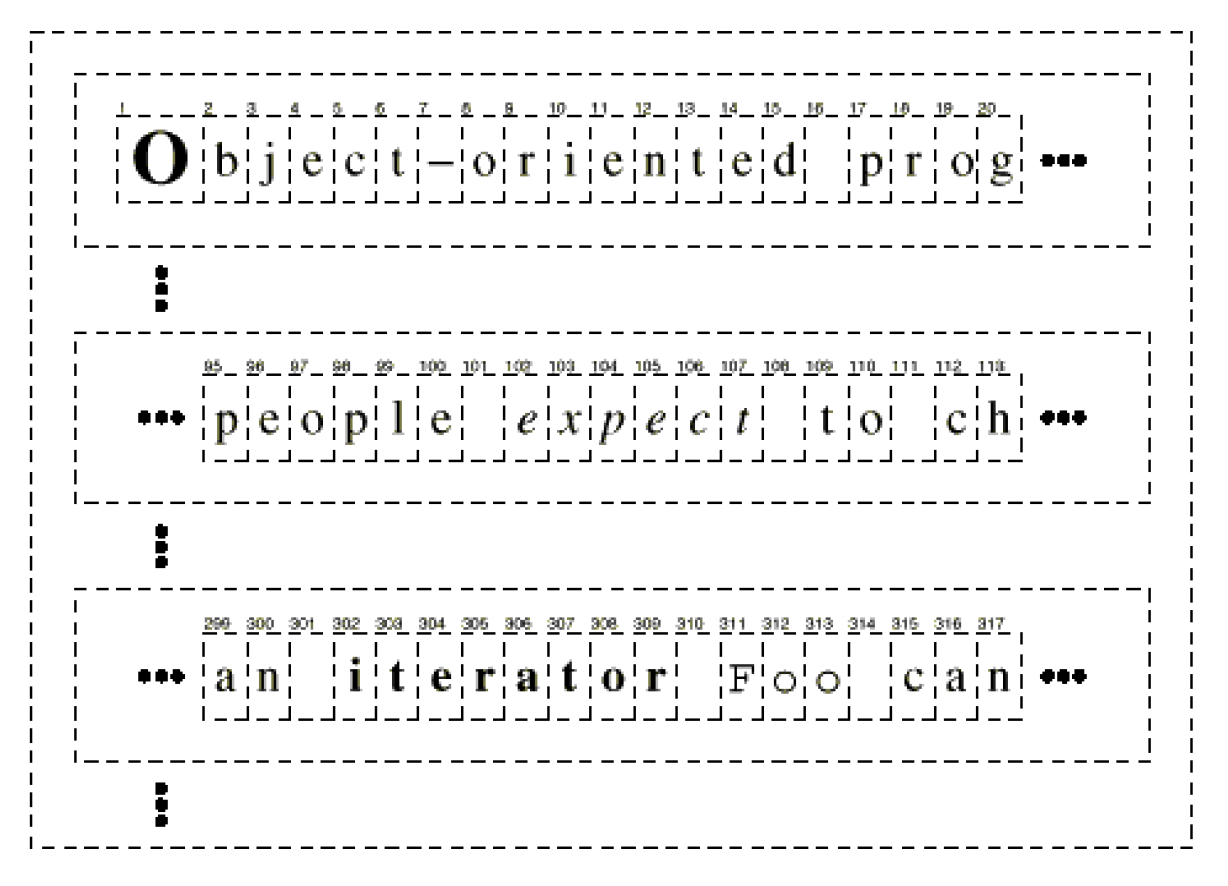
\includegraphics[scale=0.4]{example1.png}
\end{center}
\end{frame}
%-------------------------------------------------------------------------------------------------

%-------------------------------------------------------------------------------------------------
\begin{frame}\frametitle{Օրինակ}
\begin{center}
    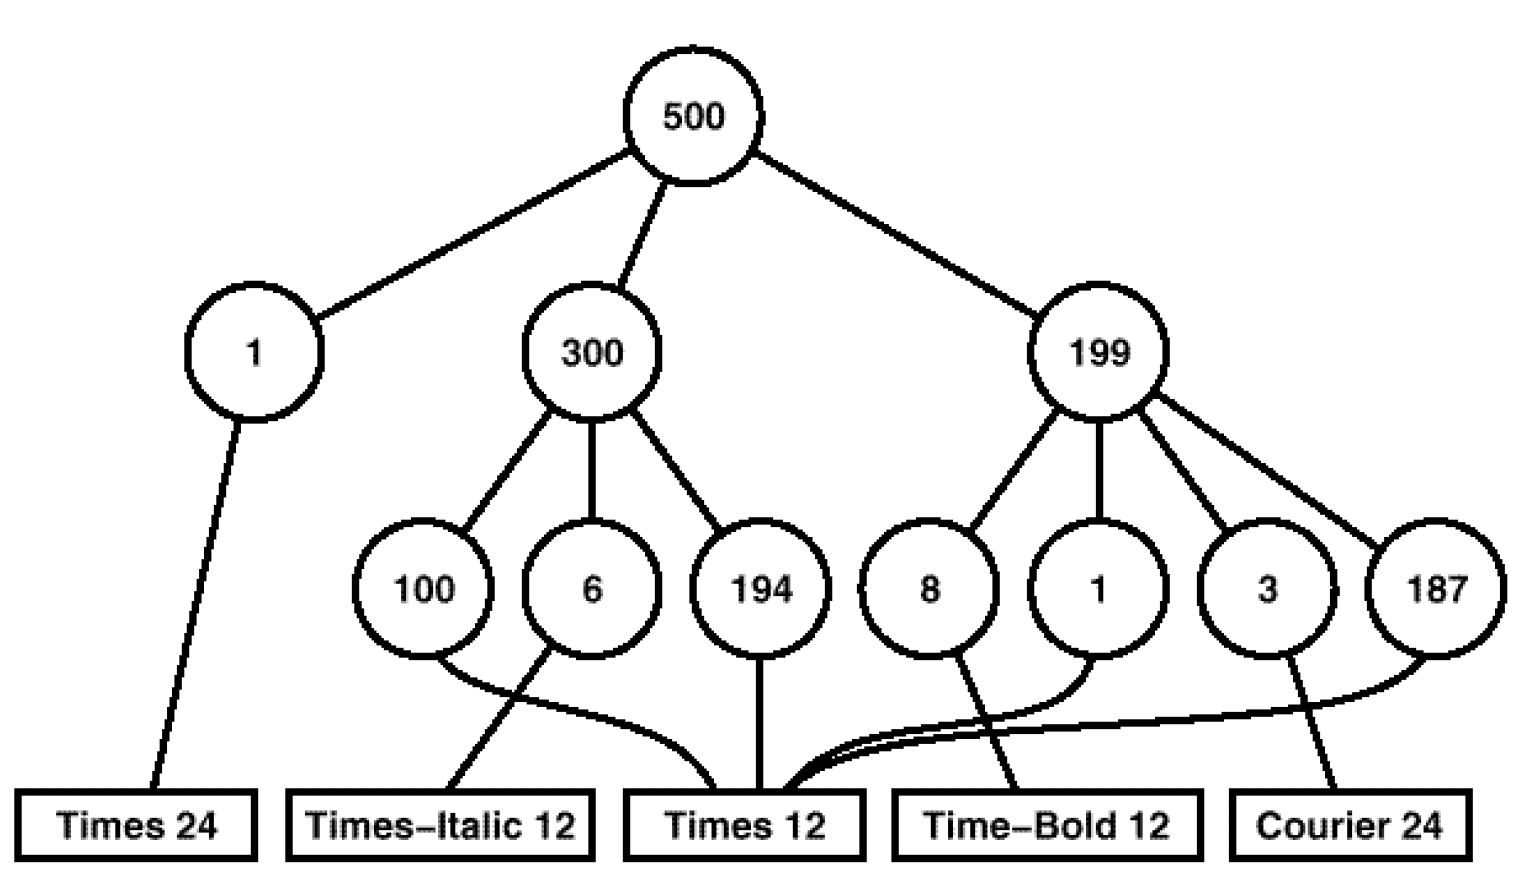
\includegraphics[scale=0.3]{example2.png}
\end{center}
\end{frame}
%-------------------------------------------------------------------------------------------------

%-------------------------------------------------------------------------------------------------
\begin{frame}\frametitle{Օրինակ}
\begin{center}
    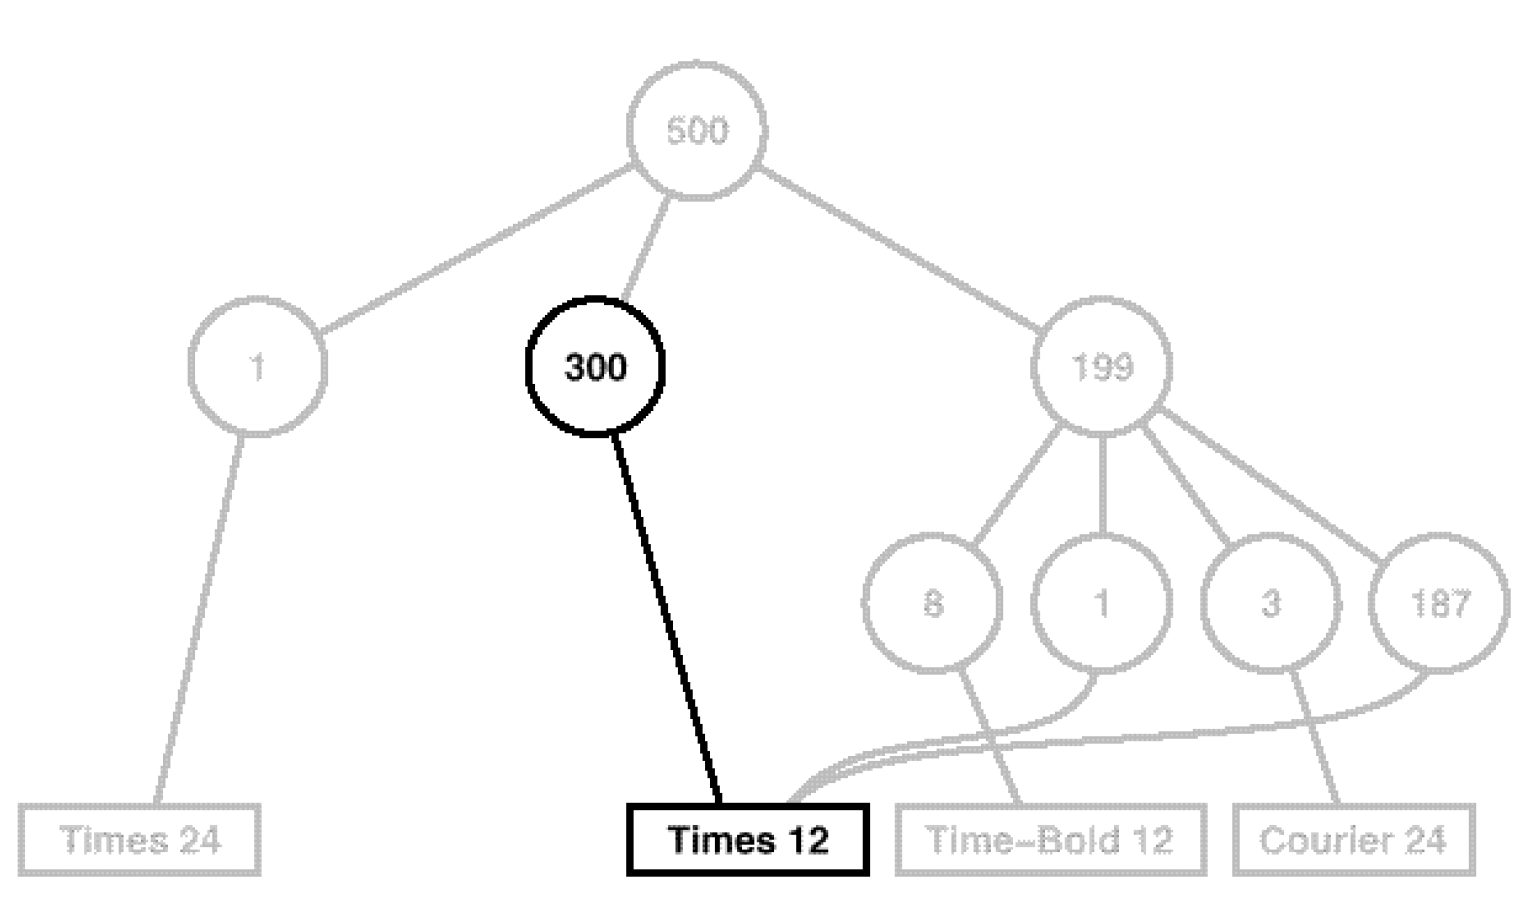
\includegraphics[scale=0.3]{example3.png}
\end{center}
\end{frame}
%-------------------------------------------------------------------------------------------------

%-------------------------------------------------------------------------------------------------
\begin{frame}\frametitle{Օրինակ}
\begin{center}
    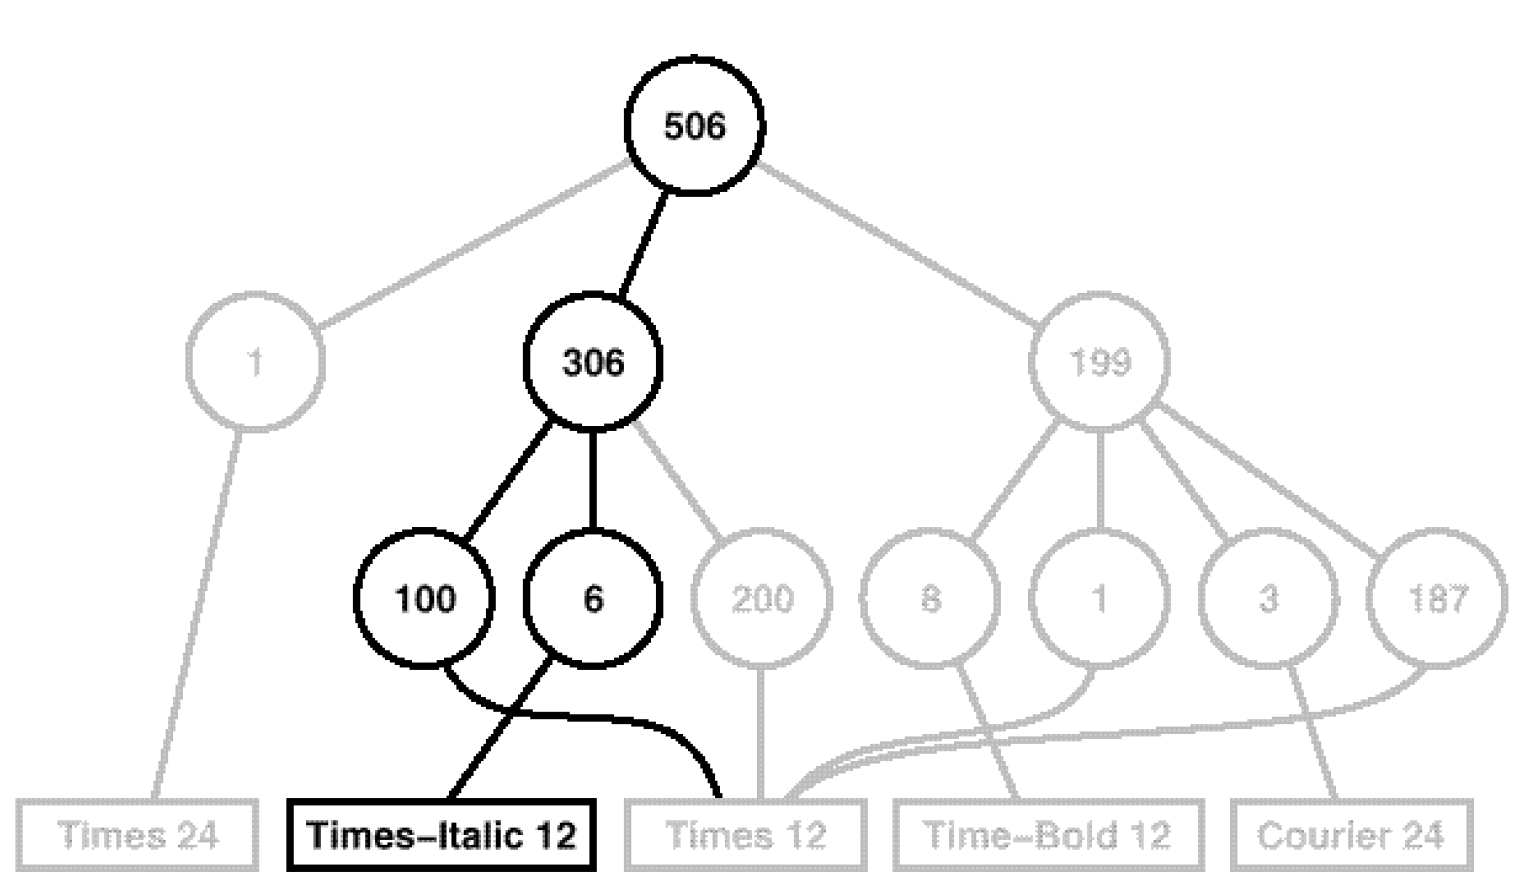
\includegraphics[scale=0.3]{example4.png}
\end{center}
\end{frame}
%-------------------------------------------------------------------------------------------------

%-------------------------------------------------------------------------------------------------
\begin{frame}[fragile]\frametitle{Օրինակ}
\begin{english}
\begin{minted}{cpp}
class GlyphFactory {

    static const int NCHARCODES = 128;

public:
    GlyphFactory();
    virtual ~GlyphFactory();
    virtual Character* CreateCharacter(char);
    virtual Row* CreateRow();
    virtual Column* CreateColumn();
    // other methods

private:
    Character* character[NCHARCODES];
};
\end{minted}
\end{english}
\end{frame}
%-------------------------------------------------------------------------------------------------

%-------------------------------------------------------------------------------------------------
\begin{frame}[fragile]\frametitle{Օրինակ}
\begin{english}
\begin{minted}[fontsize=\scriptsize]{cpp}
GlyphFactory::GlyphFactory() {
    for (int i = 0; i < NCHARCODES; ++i) {
        character[i] = 0;
    }
}

Character* GlyphFactory::CreateCharacter(char c) {
    if (!character[c]) {
        character[c] = new Character(c);
    }
    return character[c];
}

Row* GlyphFactory::CreateRow() {
    return new Row;
}

Column* GlyphFactory::CreateColumn() {
    return new Column;
}
\end{minted}
\end{english}
\end{frame}
%-------------------------------------------------------------------------------------------------

\section{Առնչվող Ձևանմուշները}
%-------------------------------------------------------------------------------------------------
\begin{frame}\frametitle{Առնչվող Նախագծման Ձևանմուշները}
\begin{itemize}
    \item Composite \vfill
    \item State \vfill
    \item Strategy
\end{itemize}
\end{frame}
%-------------------------------------------------------------------------------------------------

\end{document}
